\section{Blind Attack}
\label{sec:blindattack}

In a real-world scenario, the key is typically unknown. Therefore we do not have any information whether our best candidate is correct or not. We need some rule to recognize a fairly good candidate which we can obviously test for correctness by running AES encryption ourselves.

\begin{remark}
\label{rem:false}
	Especially note the attack against the \nth{1} byte using {\tt 3d} as a target and its last but one entry in Table \ref{tab:lintargets} -- here the incorrect candidate has a gap of almost $26\%$. It is actually the largest gap of an incorrect candidate among all targets and all bytes using this particular instance of WBAES tables. The largest gap of an incorrect candidate ever seen was almost $35\%$!
	%!% až prohodim pořadí v tabulkach tak i tady v tůtom remarku
	In our results, the target bits keep their original order (but reverse), therefore we can deduce the vector $B$ generating the target in terms of $T_B$. Here it is the second row of matrix of multiplication by $\texttt{3d}\pmod{x^8+1}$, see Example \ref{ex:shiftmatrix}. Hence the vector is $B = 01011110$.
\end{remark}

In order to perform a blind attack, we studied our results deeper, in particular we are interested in success rate of individual targets. The following section gives some of our remarks, next we suggest the blind attack itself in Section \ref{sec:subblindattack}


% ==============================================================================
% ===   R E M A R K S                                                        ===
% ==============================================================================

\subsection{Remarks}
\label{sec:remarks}

%~ We decided to create another {\tt KlinecWBAES} table instantiations in order to have larger data set. Note that for each instance we have $16$ independent tables -- one for each byte since %?% neni to podle mě uplně nezávislý ptž MC je před MB tže dycky aspon 4 byty jsou provázaný
We cannot make conclusions based on a single {\tt KlinecWBAES} table instantiation only. In order to avoid specific behavior of a single instance, we created another $7$ instances. Then we acquired $1024$ traces and ran attack against each of $16$ key bytes using all $255$ targets, for each instance. Altogether we ran $16\cdot255\cdot8=32\,640$ attacks which, together with trace acquisition and filtering, took us several hours on a regular hardware.

We processed the results and displayed several statistics, here we present some of them. Note that we only considered strong candidates as introduced in Note \ref{note:strong} (candidates with a gap greater than $10\%$).

The good news is that the overal success rate was $25\%$ (compare to $27\%$ and $31\%$ for our previous single-instance attack using the original SBox and Rijndael inverse, respectively) which gives us a hope that the new targets are successful as well. But our goal is rather to estimate individual success rate of each of our $255$ targets. (Another good news is that each target was successful at least once out of $16\cdot8=128$ chances.)

\subsubsection{Success Rate of Individual Targets}
	
	Remind that we have $255$ targets and only $8$ independent instances of tables which is quite a small data set for statistical purposes. For this reason, we rather group targets by different criteria and observe if they appear to be uniformly distributed. Note that this way we could possibly only refute uniformity, but it can still serve as reasonable justification.
	
	\paragraph{Group by corresponding $p$.}
	
	Here we make use of our former approach and group the targets by the corresponding $p$, see the transfer in Section \ref{sec:unify}. We put the results in a histogram, see Figure \ref{fig:leaktargethist}. Here we give percentual success rate for each group of targets together with their standard deviation (among $8$ measurements). Originally invertible $p$'s are in green, non-invertible in orange.
	
	\begin{figure}[h]
	\begin{center}
		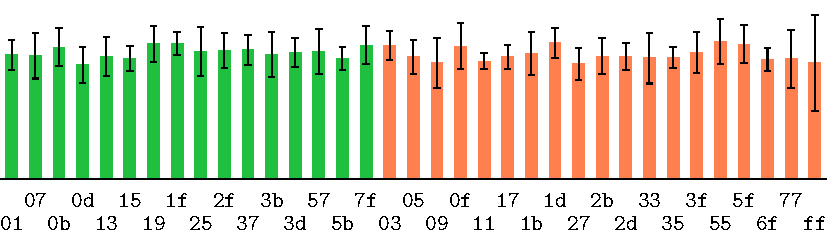
\includegraphics{figures/leak_target/leak_target.pdf}
		\caption{Success rate by targets' corresponding $p$'s and their standard deviation. Green represents invertible $p$'s, orange noninvertible ones.}
		\label{fig:leaktargethist}
	\end{center}
	\end{figure}
	
	Note high deviation at {\tt ff}, this is because there is only a single target in this group (one generated by $B^T = (1,1,1,1,1,1,1,1)$). Also note that we did not give $y$-axis scale since the purpose is only to distinguish uniform distribution.
	
	\paragraph{Group with fixed $4$ bits in $B$.}
	
	Another way of grouping we performed, groups targets by fixing $4$ out of $8$ bits of their corresponding vector $B$, see Equation \ref{eq:tba}. We fixed the first and the last $4$ bits and grouped them, see results in Figure \ref{fig:leaktargetotherhist}, where these ways of grouping are in green or orange, respectively. Group index can be computed as binary AND of mask {\tt 0xf0} or {\tt 0x0f} with vector $B$, respectively.
	
	\begin{figure}[h]
	\begin{center}
		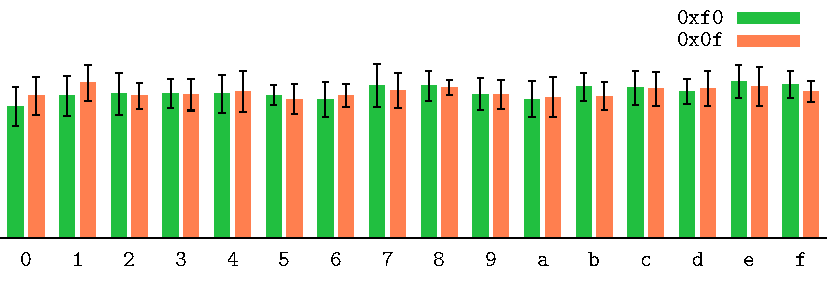
\includegraphics{figures/leak_target_other/leak_0x0f_0xf0.pdf}
		\caption{Success rate by fixed $4$ bits of targets' corresponding vector $B$. Green represents fixed first $4$ bits, orange represents last $4$ bits.}
		\label{fig:leaktargetotherhist}
	\end{center}
	\end{figure}

\subsubsection{False Positives}
	% co tu bylo:
	% average gap of correct
	% average gap of false positives
	% jak se (ne)opakujou FP
	% jak to posčítat abych nedostal žádnýho FP

\subsubsection{Using Less Traces}
	
	Note that once we use less traces, we usually do not find the correct candidate on the tail (as mentioned in Note \ref{note:tailrank}). Some results \ldots %!% results

\subsubsection{Leaking Bits}
	
	Remind that our trace is a bit-wise serialization of least significant bytes of memory addresses, hence we can identify which bit within that byte leaked -- simply by taking the leaking position within trace modulo $8$. This moduled position will be referred to as {\em leaking bit} (note the difference from target bit).
	
	We noticed soon that leaking bits are not very well balanced, therefore we put this data into a histogram, see Figure \ref{fig:leakbitall}. The histogram shows the amount of correct candidates with a gap larger than $10\%$ averaged over $8$ WBAES instances, for each leaking bit, together with standard deviation which is surprisingly very low. Note that the histogram does not provide absolute values since these could be misleading, only distribution is relevant at the moment.
	
	\begin{figure}[h]
	\begin{center}
		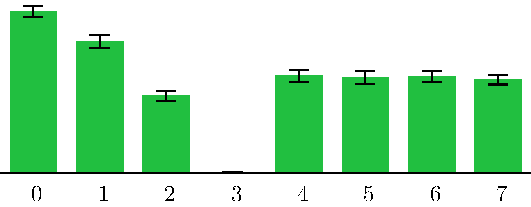
\includegraphics{figures/leak_bit/leak_bit.pdf}
		\caption{Average number of leaks and its standard deviation at each bit within trace.}
		\label{fig:leakbitall}
	\end{center}
	\end{figure}
	
	The \nth{0} and \nth{1} bits leaked slightly more, the \nth{2} bit slightly less and the \nth{3} bit actually leaked only twice while the overal average of the remaining bits was almost $160$! On the other hand, all of the remaining bits leaked fairly similarly. We do not have any explanation for this behavior.
	
	We further studied whether there is some influence of target invertibility (non-invertible targets were introduced in Section \ref{sec:noninv}).
	
	%!% že tam je furt kotel false positives, referovat, už jsem to zminoval v tom remarku myslim


% ==============================================================================
% ===   B L I N D   A T T A C K                                              ===
% ==============================================================================

\subsection{Blind Attack}
\label{sec:subblindattack}

\begin{note}
	This section only applies previous observations on a heuristic basis, there is no guarantee that our approach is the best.
\end{note}

We suggest to use less traces and repeat the attack with several targets. Even though we can hardly exploit the observation about candidates on the tail from Note \ref{note:tailrank}, it appears to be more robust and efficient to use several targets and sum the values of their respective best candidates unless filtered.

\ldots


% We rather suggest the following:
%~ \begin{enumerate}
	%~ \item pick a target, %?% Chi-square test of uniformity, pick random
	%~ \item attack using $256$ traces
%~ \end{enumerate}
% 10\% pro započtení, 75\% kumulativní mez? moc často se totiž neopakujou
% vyzkoušet jestli tak zlomim všechny instance

%~ Therefore, in case of blind attack (i.e.\ no knowledge of actual key), we suggest to use less traces, but keep changing the target until the maximal gap exceeds $27\%$, then we accept that candidate. This is likely to happen soon since $10.6$ out of $16$ targets succeed on average.

% psal já / Teuwen:
%~ > I only wonder about the reasoning why Karroumi is more than Chow since
%~ > it seems to have been shown to be equal (based on what I wrote in my
%~ > previous email).
%~ 
%~ Well I've no problem to break completely Chow with standard DCA so there
%~ is something a bit more in Karroumi. Obviously not enough to make it
%~ robust enough...
